\documentclass[12pt,a4paper,oneside]{article}
\usepackage[colorlinks=true]{hyperref}
\usepackage[utf8]{inputenc}
\usepackage[czech]{babel}
\usepackage{graphicx}
\usepackage{pdfpages}
\textwidth 16cm \textheight 25cm
\topmargin -1.3cm 
\oddsidemargin 0cm
\pagestyle{empty}
\begin{document}
\title{Emulátor digitálního syntetyzéru od DG8SAQ}
\author{Jakub Kákona, kaklik@mlab.cz}
\maketitle

\thispagestyle{empty}
\begin{abstract}
Vzhledem k tomu, že je potřebné modul CLKGEN01B nějakým způsobem přelaďovat, je vhodné jej připojit například k počítači. Tento článek popisuje způsob, jak ovládat čip Si570 pomocí sběrnice USB. 
\end{abstract}

\begin{figure} [htbp]
\begin{center}
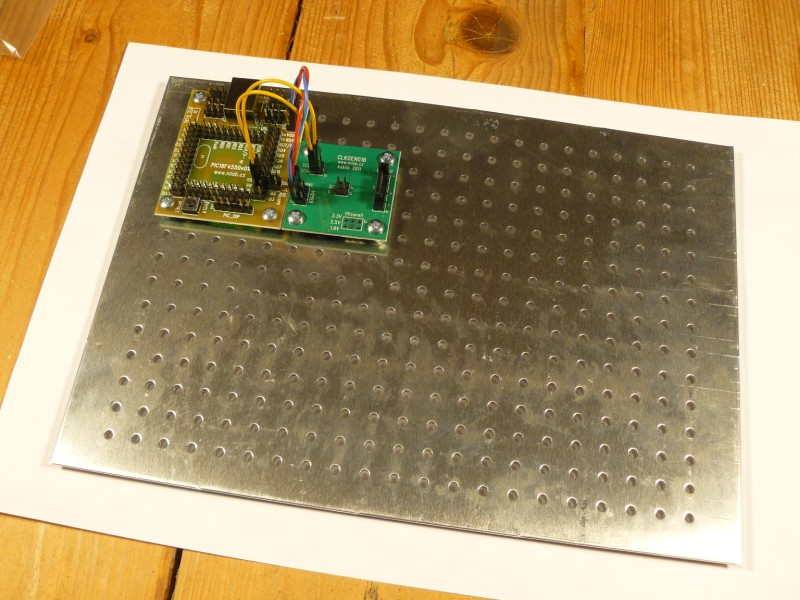
\includegraphics [width=80mm] {DG8SAQ_emulator_Big.jpg} 
\end{center}
\end{figure}

\tableofcontents

\section{Technické parametry}
\begin{table}[htbp]
\begin{center}
\begin{tabular}{|c|c|p{4.7cm}|}
\hline
Parametr & Hodnota & Poznámka \\
\hline
Napájecí napětí POWER  & max 5V &  Napájení z USB\\ 
\hline
Frekvenční rozsah  & 10 - 1500 MHz & Záleží na konkrétním typu čipu Si5XX, obvykle 10-810MHz \\ 
\hline
Fázový jitter  & $<$ 0,3ps & Pro obvody řady Si570 z diferenciálním výstupem\\ 
\hline
\end{tabular}
\end{center}
\end{table}

\section{Popis konstrukce}
Zařízení vychází z velmi rozšířené metody ovládání čipu Si570 pomocí ATtiny, tak jak byla navžena v . Tento postup funguje, ale díky nekompatibilním napěťovým úrovním na USB a na ATtiny, může způsobovat nežádoucí rušení. Navíc v některých moderních implementacích USB 3.0 může být jeho použití rizikové pro host zařízení v počítači. Zde je tedy popsán technicky mnohem čistčí způsob vyhovující standardu USB při zachování všech funkcí původní konstrukce.
Navíc je zde i korektně bezodrazově vyšešen vysokofrekvenční výstup z čipu Si570. 

\subsection{Zapojení}
Zapojení spočívá pouze v propojení modulu PIC18F4550v01A s modulem CLKGEN01B. Toto je realizováno jedním napájecím kablíkem, který propojuje napájení modulu připojeného na USB s 5V napájením CLKGEN01B (Modul si nižší napájecí napětí stabiluzuje sám). V zapojení jsou ještě dva datové kablíky, které přímo propojují I2C sběrnici.
Na modulu PIC18F4550v01A je jako napájení jumperem zvoleno USB. Použitý krystal je 20 MHz

\subsection{Odrušení}

Odrušení je třeba provádět zvláště pečlivě, pracujeme-li v prostředí, kde by mohlo vadit elektromagnetické vyzařování, jako je například radioastronomie. Nejkritičtějším místem je v tomto případě připojení počítače, který je často sám o sobě silným zdrojem rušení. USB kabel je tedy vhodné volit dostatečně stíněný a nejlépe s odrušovacími ferity na obou koncích. Počítač by sám o sobě měl do USB injektovat co nejmenší množství šumu, proto je dobré použít místo notebooku spíše stolní počítač s kvalitním zdrojem a kovovou bednou. Samozřejmost je mít moduly přišroubované na dostatečně vodivé podložce tedy nejlépe ALBASE.  

\section{Nastavení testování}
Při připojení k napájení generuje CLKGEN01B frekvenci nastavenou při výrobě v Silicon Labs. Pro možnost ladění je potřeba do PIC18F4550 nahrát firmware, který naleznete na . Při úspěšném nahrání firmwaru programátorem například PICprogUSB02A, se sestava připojením k počítači ohlásí jako nové USB zařízení a bude vyžadovat driver. Ten lze ten je stejný jakopro původní konstrukci a lze jej nalézt v odkazu.

\section{Programové vybavení}
Vzhledem k tomu, že výsledek je plně kompatibilní s  \cite{DG8SAQSynthesizer} lze k ladění generátoru použít naprostou většinu programů pro SDR a nebo pouze pro nastavení frekvence například USBSynth \cite{USB_Synth}.

\begin{thebibliography}{99}
\bibitem{Si570board}{Původní konstrukce Si570 Board } 
\href{http://wb6dhw.com/inactive.html}{http://wb6dhw.com/inactive.html}

\bibitem{DG8SAQemulator}{PIC emulátor USB syntezátoru od DG8SAQ} 
\href{http://www.qrpradio.org/pub/softrocks/manuals/Softrock Group Files 210109/21 9V1AL/02 UBW Emulator/README.txt}{http://www.qrpradio.org/pub/softrocks/manuals/Softrock Group Files 210109/21 9V1AL/02 UBW Emulator/README.txt}

\bibitem{DG8SAQSynthesizer}{Wideband RF Synthesizer} 
\href{http://www.mydarc.de/dg8saq/SI570/index.shtml}{http://www.mydarc.de/dg8saq/SI570/index.shtml}

\bibitem{USB_Synth}{USB Synth}
\href{ http://www.mydarc.de/dg8saq/hidden/USB\_Synth3.zip}{http://www.mydarc.de/dg8saq/hidden/USB\_Synth3.zip}

\end{thebibliography}
\end{document}